\documentclass[10pt,a4paper]{article}


%% the github permalink is at https://damjanmiklos.github.io/cv/main.pdf

% ==========================================
% PACKAGES & SETUP
% ==========================================
\usepackage[utf8]{inputenc}
\usepackage[T1]{fontenc}
\usepackage[english]{babel}
\usepackage[margin=1.0cm]{geometry}
\usepackage{helvet}
\renewcommand{\familydefault}{\sfdefault}
\usepackage{fontawesome5}
\usepackage{paracol}
\usepackage{graphicx}
\usepackage{xcolor}
\usepackage{enumitem}
\usepackage{hyperref}
\usepackage{ragged2e}

% ==========================================
% CUSTOM FORMATTING
% ==========================================

\pagestyle{empty}

\definecolor{accent}{RGB}{0,62,116}
\definecolor{subtle}{RGB}{90,90,90}

\hypersetup{
    unicode=true,
    pdfnewwindow=true,
    colorlinks=true,
    linkcolor=black,
    citecolor=black,
    urlcolor=accent,
    pdftitle={Damján Miklós -- CV},
    pdfauthor={Damján Miklós}
}

% ==========================================
% COLUMN CONFIGURATION
% ==========================================
% Narrow sidebar for short lists, wide main column for entries with bullets
\columnratio{0.29}
\setlength{\columnsep}{1.4em}

% Section header: accent-coloured title with a thin rule
\newcommand{\cvsection}[1]{%
    \vspace{0.32cm}%
    {\color{accent}\large\bfseries #1}\par\vspace{0.06cm}%
    {\color{accent}\hrule height 0.6pt}\vspace{0.16cm}%
}

% Sidebar sub-heading
\newcommand{\sidehead}[1]{{\bfseries #1}\par\vspace{1pt}}

% ==========================================
% CUSTOM COMMANDS
% ==========================================

% Entry: {Title}{Date}{Institution}{Body}
\newcommand{\cventry}[4]{%
    {\bfseries #1}\hfill{\small\color{subtle}#2}\par
    {\itshape #3}\par
    \vspace{1pt}%
    #4%
    \par\vspace{0.2cm}%
}

% Dated list line: {Year}{Text}, year in a fixed-width left gutter
\newcommand{\cvaward}[2]{%
    \item[{\small\color{subtle}#1}] #2
}
\newenvironment{datedlist}{%
    \begin{itemize}[leftmargin=2.6em, labelwidth=2.2em, labelsep=0.4em, align=left]%
}{\end{itemize}}

\setlist[itemize]{leftmargin=1em, label={\color{accent}\textbullet}, noitemsep, topsep=1pt, parsep=0pt}

% ==========================================
% DOCUMENT START
% ==========================================
\begin{document}

\RaggedRight

\begin{paracol}{2}

% ====================
% LEFT COLUMN (sidebar)
% ====================

\begin{center}
    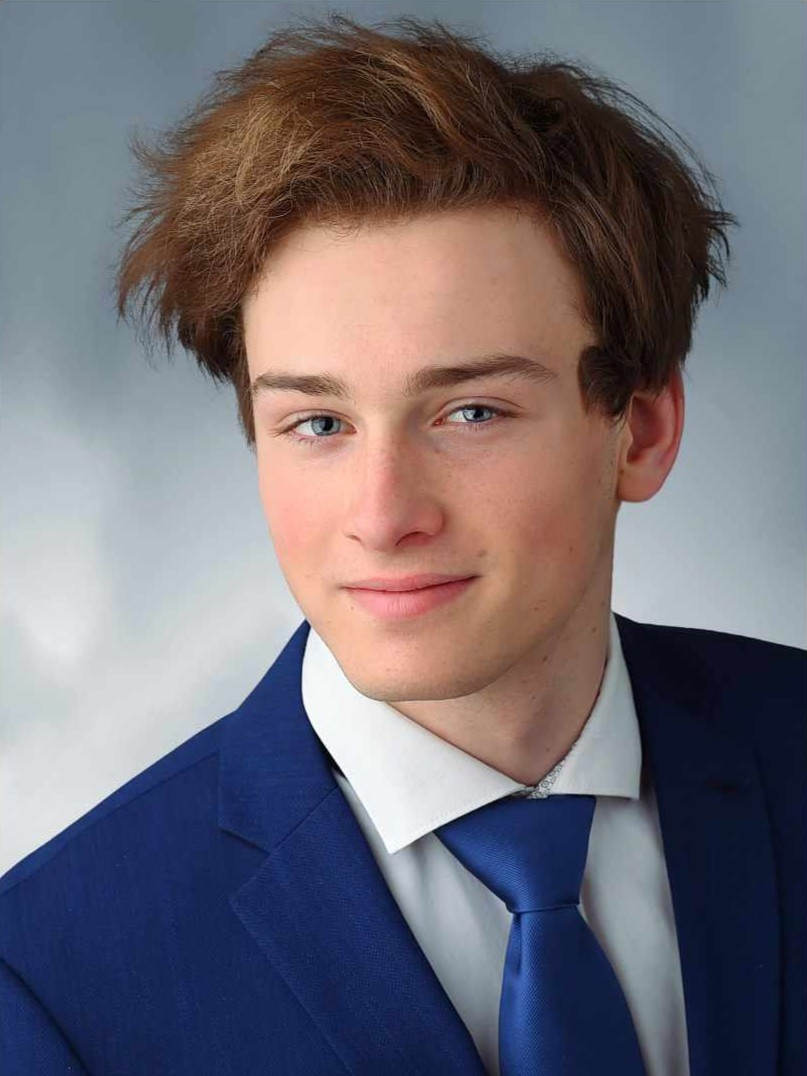
\includegraphics[width=3.3cm, keepaspectratio]{profile_pic.jpg}
\end{center}

\vspace{0.1cm}

{\small
\begin{tabular}{@{}c@{\hspace{0.5em}}l@{}}
    \faAt & \href{mailto:damjan.miklos@gmail.com}{damjan.miklos@gmail.com} \\
    \faMobile* & +36 30 792 9424 \\
    \faLinkedin & \href{https://www.linkedin.com/in/damjan-miklos/}{linkedin.com/in/damjan-miklos} \\
    \faGraduationCap & \href{https://scholar.google.com/citations?user=lAZQuOQAAAAJ&hl=en}{Google Scholar} \\
    \faGithub & \href{https://github.com/damjanmiklos}{github.com/damjanmiklos}
\end{tabular}
}

\cvsection{Skills}

\sidehead{ML \& Data}
PyTorch, graph neural networks, image segmentation, uncertainty quantification (Dakota), SQL

\vspace{0.15cm}
\sidehead{Programming}
Python, MATLAB, C, C++, R, TypeScript/React, Wolfram Mathematica, Solidity

\vspace{0.15cm}
\sidehead{Engineering}
AutoCAD, Inventor, LabVIEW, MPLAB

\vspace{0.15cm}
\sidehead{Tools}
Git, Linux (WSL), HPC, Jupyter, \LaTeX

\cvsection{Languages}

\textbf{Hungarian:} native \\
\textbf{English:} C1 (IELTS) \\
\textbf{German:} B2 \\
\textbf{French:} B1

\cvsection{Interests}

Ultra-endurance cycling \\
Drumming \\
PC hardware \& overclocking \\
DIY -- built a garden house


\switchcolumn

% ====================
% RIGHT COLUMN (main)
% ====================

{\Huge\bfseries Damján \textcolor{accent}{MIKLÓS}}\par
\vspace{0.15cm}
{\large Mechatronics Engineering BSc student}\par
\vspace{0.05cm}
{\color{subtle} Machine learning and uncertainty quantification for cardiovascular simulation}\par

\cvsection{Education}

\cventry{BSc in Mechatronics Engineering}{Sep 2023 -- Jan 2027 (expected)}
{Budapest University of Technology and Economics (BME)}
{GPA: \textbf{4.7/5} \quad$\cdot$\quad Advanced Mathematics Program \quad$\cdot$\quad Specialization: Analysis of Mechatronic Structures}

\textbf{Guest Student}, ELTE Faculty of Science \hfill{\small\color{subtle}Spring 2023}\par
Fourier Analysis lectures by special permission while in high school\par
\vspace{0.2cm}
\textbf{High School Diploma}, ELTE Trefort Ágoston High School \hfill{\small\color{subtle}2017 -- 2023}\par
Specialization in Mathematics, Physics and English\par

\cvsection{Publications \& Presentations}

\textbf{Miklós, D.} (2026). Irrationality in skewness preferences. \textit{Finance Research Letters}, 109, 110514.
\href{https://doi.org/10.1016/j.frl.2026.110514}{doi:10.1016/j.frl.2026.110514}
\textit{-- sole author, Scopus D1 journal}

\vspace{0.12cm}
\textbf{Oral presentation}, VPH 2026 Conference (Virtual Physiological Human), Milan\par
\textbf{Oral presentation}, CMFF 2025 (Conference on Modelling Fluid Flow), Budapest\par
{\small\color{subtle}Both talks: comparison of uncertainty quantification methods for aneurysm hemodynamics}

\cvsection{Research Experience}

\cventry{Research Assistant}{Nov 2024 -- present}
{BME Department of Hydrodynamic Systems}
{\begin{itemize}
    \item Developing a conditional generative graph neural network that creates anatomically accurate internal carotid artery (ICA) meshes with aneurysms from a single condition vector, including cleaning and preprocessing of high-resolution meshes in Python \textit{(BSc thesis)}
    \item Developing a neural network for segmenting calcified ICAs
    \item Compared uncertainty quantification methods for aneurysm hemodynamics simulations using Dakota, Python and MATLAB
    \item Built an efficient virtual patient sampling algorithm in MATLAB
\end{itemize}}

\cventry{Independent Research, Empirical Finance}{2024 -- 2026}
{BME Department of Finance}
{\begin{itemize}
    \item Built a model-independent, distribution-based benchmark showing that the equity skewness premium exceeds its rational upper bound, pointing to behavioural drivers
\end{itemize}}

\cvsection{Selected Awards}

\begin{datedlist}
    \cvaward{2026}{\textbf{1st Place}, EELISA Scientific Student Competition, Madrid (international)}
    \cvaward{2026}{\textbf{xxx Place}, BME Scientific Students' Conference -- generative GNN}
    \cvaward{2025}{\textbf{1st Place} + GHK Special Award, BME Scientific Students' Conference -- UQ}
    \cvaward{2025}{\textbf{3rd Place}, National Scientific Students' Conference (OTDK) -- finance}
    \cvaward{2024}{\textbf{1st Place} + Morgan Stanley Award, BME Scientific Students' Conference}
\end{datedlist}

\cvsection{Other Experience \& Projects}

\textbf{Online Math \& Physics Tutor}, \href{https://www.superprof.hu/mechatronikus-hallgatokent-barkit-szivesen-tanitok-matek-fizikara-online-eddigi-ertekeleseim-alapjan-egyik-legjobban.html}{Superprof} \hfill{\small\color{subtle}2023 -- present}\par
2000+ hours of university-level tutoring in English and Hungarian; among the top-rated tutors nationwide\par
\vspace{0.2cm}

\textbf{\href{https://github.com/damjanmiklos/dynamicspeed-for-youtube}{DynamicSpeed for YouTube}} \hfill{\small\color{subtle}2026}\par
Chrome/Firefox extension that matches playback speed to a target words-per-minute\par

\end{paracol}
\end{document}
